\documentclass[10pt,a4paper]{report}
\usepackage[latin1]{inputenc}
\usepackage{amsmath}
\usepackage{amsfonts}
\usepackage{amssymb}
\usepackage{graphicx}
\title{matrixIxirtam\\$\mid$\\$matrixi$: an open project for\\camera synchronisation check}
\author{Sebastien COUDERT}
\begin{document}
\maketitle
\tableofcontents

\chapter{matrixIxirtam}
\section{description}
\begin{itemize}
\item aim: \textbf{check multiple camera synchronisation}.
\item solution: simply based on imaging a number that is changing in time.
\item constrain: \textbf{fast and reliable processing}. easy implementation.
\end{itemize}
\subsection{no number as characters}
no OCR: too complex and too slow.
parallel to conversion from binary to ASCII (and vice versa) = lot of CPU time.
\subsection{number as matrix}
digital number = bits.
use \textbf{16 light spots to create 16 bit number}.
16 light spots layout on a \textbf{4x4 matrix} (i.e. 2D array).
image processing is simple: get bits on image:
\begin{itemize}
\item high level = 1 = true
\item low level = 0 = false
\end{itemize}
matrix layout as:\\
0 0 0 0\\
0 0 0 0\\
0 0 0 0\\
0 0 0 0\\
For example, number 123 (i.e. 0000 0000 0111 1011 as binary) will show as follow in \textbf{image axis convention}:\\
1 1 0 1\\
1 1 1 0\\
0 0 0 0\\
0 0 0 0\\
easy implementation in C++ or GHDL language.
\subsection{project name}
Project is nicknamed $matrixi$ for easy prononciation.
The full name is $matrixIxirtam$ 
to stand for a given number
that is converted to a matrix
then it is convert back to number.
One way is $matrix$ the reverse way is $xirtam$ (i.e. \textbf{reverse order} characters of matrix).
It is a kind of mirroring:
i as a capital letter stands for $\mid$ which represent the \textbf{mirror} (i.e. matrixIxirtam).
This name is easy to write as text (e.g. Linux terminal or C++ code) or render as a figure (e.g. XWindows display or LaTeX).

\section{component}
\begin{figure}
  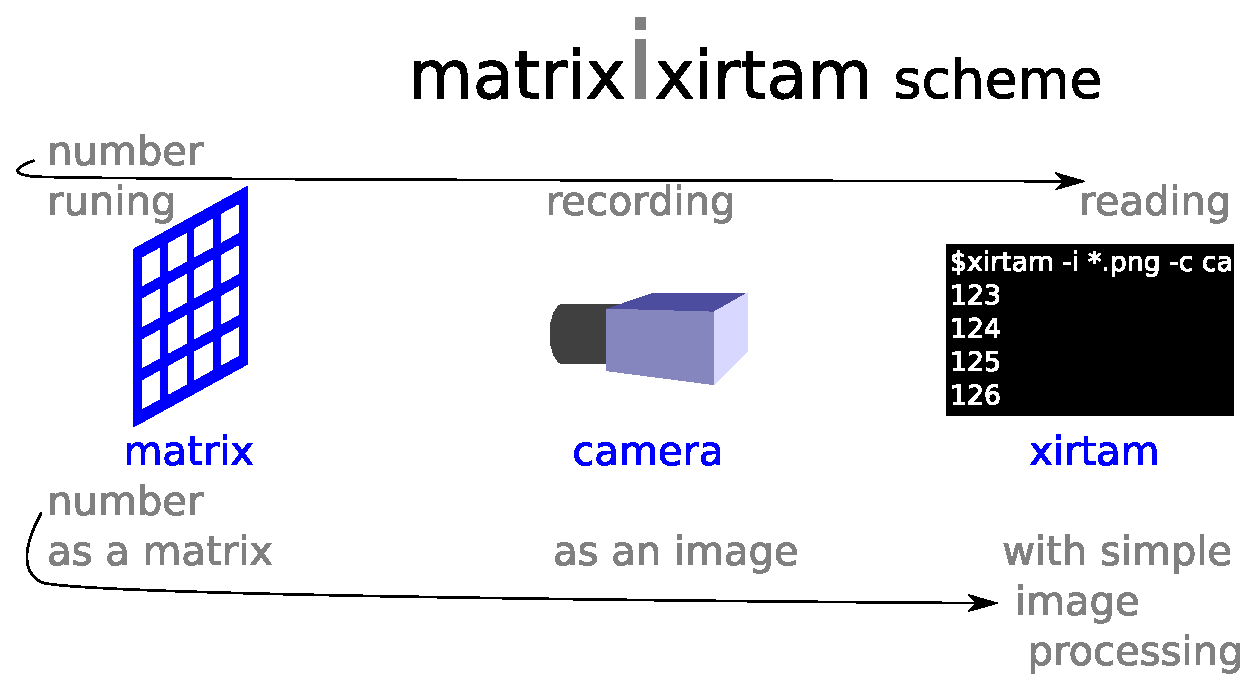
\includegraphics[width=0.95\textwidth]{figure/matrixIxirtam.eps}
  \caption{matrixIxirtam overview}
  \label{fig:matrixIxirtam_scheme}
\end{figure}
\subsection{description}
The components of the project layout on the figure~\ref{fig:matrixIxirtam_scheme}.
\begin{enumerate}
\item The number is displayed as a light spot matrix using a device called \textbf{$matrix$ component} in the project.
\item The image of the matrix is recorded using one (or multiple) camera but which is not part of the project.
\item The images are processed using the \textbf{$xirtam$ component}, that decodes the number.
\end{enumerate}
To comment on each step again:
\begin{enumerate}
\item $matrix$ component is creating a number incremented in time (either software or hardware delay). For example, the number begins at 123 (i.e. 0000 0000 0111 1011 as binary or bit matrix) for first image, then after the delay it is 124 (i.e. 0000 0000 0111 1110) for second image and so on.
\item multiple cameras may be able to record images of the same $matrix$ component to record same times (i.e. same number as a matrix; e.g. 124 for all second images of cameras).
\item $xirtam$ component is reading the numbers (e.g. 123,124,125,126,...) and may compare it either from preceeding or following one (e.g. 123,124,125) and in between cameras at the same image index (e.g. 124), to check for synchronisation.
\end{enumerate}
note: 
fast image processing (real time).
no complex OCR.
\subsection{matrix}
write number as a matrix. 16 light spots.
different ways of making the matrix image.
examples
\begin{itemize}
\item display on a computer screen (see section~\ref{CImg.matrix} $CImg.matrix$)
\item LED display controled by a microcontroler (see section~\ref{LED.matrix} $LED.matrix$)
\end{itemize}
use depending on accuracy and speed.
\subsection{xirtam}
read number from the recorded image using the matrix image.
different ways of converting the matrix image to the corresponding number.
examples
\begin{itemize}
\item sequence of previously recorded images (see section~\ref{CImg.xirtam} $CImg.xirtam$)
\item real time reading (see section~\ref{OpenCV.xirtam} $OpenCV.xirtam$)
\end{itemize}

\chapter{matrix}
\section{CImg.matrix}\label{CImg.matrix} 
based on CImg library.
display the matrix image on the computer screen that is runnning the program.
stand alone component, but display images of the running number with a millisecond accuracy.
see doxygen documentation
\begin{itemize}
\item user
\item developper
\end{itemize}
\section{LED.matrix}\label{LED.matrix} 
actually under implementation.
16 LED for number as a matrix (i.e. 16 bit number incremented at the end each period time).
03 LED for axes markers (always on).
(01 LED for exposure)
not stand alone component: it need to be controled by an other device such as $AVR.matrix$ or $ARM.matrix$.
\subsection{LED.matrix single sided}
\subsection{LED.matrix double sided}
\section{AVR.matrix}
future implementation on an AVR microcontroler using a LED.matrix.
e.g. Arduino Mega.
\section{ARM.matrix}
future implementation on an ARM microcontroler using a LED.matrix
e.g. LeafLabs Maple.

\chapter{image recording}
\section{independant}
record images with thrid party software.
\section{part of xirtam}
record images with matrixIxirtam project software.
future implementation (see for example section~\ref{OpenCV.xirtam} $OpenCV.xirtam$)

\chapter{xirtam}
3 main steps in $xirtam$ component:
\begin{enumerate}
\item first, calibration procedure to get position within the image of the matrix on the field of view, and also values for both minimum and maximal gray levels that corresponds to low and high level of the bit. It require once the user interaction through a GUI (e.g. XWindows) on a single image per camera. This may be saved in a file for future use if neither the camera nor the matrix component are moving.
\item then, read number using simple image processing from the recorded images.This may be run in batch mode using a calibration file.
\item finally, compare numbers to a reference and/or in between cameras.
\end{enumerate}
\section{CImg.xirtam}\label{CImg.xirtam} 
based on CImg library.
read standard image format.
specifications:
\begin{itemize}
\item handle multiple cameras in only one program call.
\item run either in GUI or batch modes.
\end{itemize}
see doxygen documentation
\begin{itemize}
\item user
\item developper
\end{itemize}
\section{OpenCV.xirtam}\label{OpenCV.xirtam} 
future implementation using OpenCV/GStreamer.
may: record (through GStreamer) and process in real time.
\section{Elphel.xirtam}
future implementation using either embedded FPGA and/or ARM.
may: record and process in real time, outputting embedded Linux date and corresponding number for each camera.

\end{document}
